\documentclass[letterpaper,10pt,conference]{ieeeconf}

\IEEEoverridecommandlockouts % \thanks command
\overrideIEEEmargins % Needed to meet printer requirements.

\usepackage[pdftex]{graphicx} % for pdf, bitmapped graphics files
\graphicspath{ {figures/} }

\usepackage{epsfig} % for postscript graphics files
%\usepackage{mathptmx} % assumes new font selection scheme installed
%\usepackage{times} % assumes new font selection scheme installed
\usepackage[table,xcdraw,usenames,dvipsnames]{xcolor}
\usepackage[utf8]{inputenc}
\usepackage{amsmath}
\usepackage{amssymb}
\usepackage{bm}
\usepackage{cite}
\usepackage{url}
\usepackage{booktabs}
\usepackage{multirow}
\usepackage{adjustbox}
% \usepackage{subcaption}

\newcommand*{\skinny}[1]{{
\medmuskip=0mu\relax
\thickmuskip=0mu\relax
\small#1}}

\newcommand{\sign}{\operatorname{sign}}

\newcommand*{\of}[1]{\ensuremath{(#1)}}
\newcommand*{\inverseof}[1]{\ensuremath{\of{#1}\inverse}}

\newcommand*{\vect}[1]{\ensuremath{\bm{\mathrm{#1}}}}
\newcommand*{\mat}[1]{\ensuremath{\bm{\mathrm{#1}}}}

\newcommand*{\modvar}[2][]{\ensuremath{#1{#2}}}
\newcommand*{\modvect}[2][]{\ensuremath{\modvar[#1]{\vect{#2}}}}
\newcommand*{\modmat}[2][]{\ensuremath{\modvar[#1]{\mat{#2}}}}

\newcommand*{\at}[2]{\ensuremath{\left. {#1} \right\vert_{#2}}}

\newcommand*{\half}{\ensuremath{\frac{1}{2}}}

% modifiers
\newcommand*{\hatdot}[1]{\ensuremath{\dot{\hat{#1}}}}
\newcommand*{\inverse}{\ensuremath{{}^{-1}}}

% operators
\newcommand*{\transpose}{\ensuremath{\mathsf{T}}}
\newcommand*{\norm}[1]{\left\lVert#1\right\rVert}
\newcommand*{\skewmat}[1]{\left\lfloor#1\right\rfloor}
\newcommand*{\pard}[2]{\frac{\partial {#1}}{\partial {#2}}}

% unit vectors
\newcommand*{\ii}[1][]{\modvect[#1]{i}}
\newcommand*{\jj}[1][]{\modvect[#1]{j}}
\newcommand*{\kk}[1][]{\modvect[#1]{k}}
\newcommand*{\g}[1][]{\modvect[#1]{g}}
\newcommand*{\f}[1][]{\modvect[#1]{f}}
\newcommand*{\n}[1][]{\modvect[#1]{n}}

% quaternions
\newcommand*{\quatvec}[2][]{\modvect[#1]{\bar{#2}}}
\newcommand*{\quatscalar}[2][]{\modvar[#1]{#2}_0}

\newcommand*{\0}[1][]{\modvect[#1]{0}}
\newcommand*{\p}[1][]{\modvect[#1]{p}}
\newcommand*{\pvec}[1][]{\quatvec[#1]{p}}
\newcommand*{\pw}[1][]{\quatscalar[#1]{p}}

\newcommand*{\q}[1][]{\modvect[#1]{q}}
\newcommand*{\qvec}[1][]{\quatvec[#1]{q}}
\newcommand*{\qw}[1][]{\quatscalar[#1]{q}}

\newcommand*{\dq}[1][]{\delta\modvect[#1]{\q}}

% vectors
\newcommand*{\y}[1][]{\modvect[#1]{y}}
\renewcommand*{\v}[1][]{\modvect[#1]{v}}
\newcommand*{\dv}[1][]{\delta\modvect[#1]{v}}
\renewcommand*{\u}[1][]{\modvect[#1]{u}}
\renewcommand*{\g}[1][]{\modvect[#1]{g}}
\newcommand*{\z}[1][]{\modvect[#1]{z}}
\renewcommand*{\r}[1][]{\modvect[#1]{r}}
\newcommand*{\dth}[1][]{\delta\modvect[#1]{\theta}}

\newcommand*{\dtht}[1][]{\Delta\modvect[#1]{\theta}}

% matrices
\newcommand*{\I}{\mat{I}}
\newcommand*{\R}{\mat{R}}
\newcommand*{\Rt}{\R^\transpose}
\renewcommand*{\P}[1][]{\modmat[#1]{P}}
\newcommand*{\F}{\mat{F}}
\newcommand*{\G}{\mat{G}}
\newcommand*{\Q}{\mat{Q}}
\renewcommand*{\H}{\mat{H}}
\newcommand*{\K}{\mat{K}}
\newcommand*{\M}{\mat{M}}

\newcommand*{\N}{\mat{N}}
\newcommand*{\Np}{\mat{N}_{\vect{p}}}
\newcommand*{\Nth}{\mat{N}_{\vect{\theta}}}

% Misc
\renewcommand{\t}{t}
\newcommand{\up}{\string^}
\newcommand{\down}{\string^}

\newcommand*{\ay}[1][]{\prescript{a}{}{\y}}
\newcommand*{\by}[1][]{\prescript{b}{}{\y}}
\newcommand*{\cy}[1][]{\prescript{c}{}{\y}}

% state
\newcommand*{\x}[1][]{\modvect[#1]{x}}

\newcommand*{\pnb}[1][]{{\modvect[#1]{p}_n^b}}
\newcommand*{\pnnb}[1][]{{\prescript{n}{}{\modvect[#1]{p}}_n^b}}
\newcommand*{\pbn}[1][]{{\modvect[#1]{p}_b^n}}
\newcommand*{\pbbn}[1][]{{\prescript{b}{}{\modvect[#1]{p}}_b^n}}
\newcommand*{\pnk}[1][]{{\modvect[#1]{p}_n^k}}
\newcommand*{\pnnk}[1][]{{\prescript{n}{}{\modvect[#1]{p}}_n^k}}
\newcommand*{\pkn}[1][]{{\modvect[#1]{p}_k^n}}
\newcommand*{\pkkn}[1][]{{\prescript{k}{}{\modvect[#1]{p}}_k^n}}
\newcommand*{\pbc}[1][]{{\modvect[#1]{p}_b^c}}
\newcommand*{\pkkc}[1][]{{\modvect[#1]{p}_k^{kc}}}
\newcommand*{\pkcc}[1][]{{\modvect[#1]{p}_{kc}^c}}
\newcommand*{\pckc}[1][]{{\modvect[#1]{p}_c^{kc}}}
\newcommand*{\pabc}[1][]{{\prescript{c}{}{\modvect[#1]{p}}_a^b}}
\newcommand*{\pab}[1][]{{\modvect[#1]{p}_a^b}}
\newcommand*{\pkc}[1][]{{\modvect[#1]{p}_k^{kc}}}

\newcommand*{\qnb}[1][]{{\modvect[#1]{q}_n^b}}
\newcommand*{\qbn}[1][]{{\modvect[#1]{q}_b^n}}
\newcommand*{\qnk}[1][]{{\modvect[#1]{q}_n^k}}
\newcommand*{\qkn}[1][]{{\modvect[#1]{q}_k^n}}
\newcommand*{\qbc}[1][]{{\modvect[#1]{q}_b^c}}
\newcommand*{\qkkc}[1][]{{\modvect[#1]{q}_k^{kc}}}
\newcommand*{\qkcc}[1][]{{\modvect[#1]{q}_{kc}^c}}
\newcommand*{\qckc}[1][]{{\modvect[#1]{q}_c^{kc}}}
\newcommand*{\qab}[1][]{{\modvect[#1]{q}_a^b}}
\newcommand*{\qba}[1][]{{\modvect[#1]{q}_b^a}}
\newcommand*{\qac}[1][]{{\modvect[#1]{q}_a^c}}
\newcommand*{\vb}[1][]{{\modvect[#1]{v}}}
\newcommand*{\dthnb}[1][]{{\dth[#1]_n^b}}
\newcommand*{\dthnk}[1][]{{\dth[#1]_n^k}}
\newcommand*{\dthkn}[1][]{{\dth[#1]_k^n}}
\newcommand*{\dthbn}[1][]{{\dth[#1]_b^n}}

\newcommand*{\angvel}[1][]{\modvect[#1]{\omega}}
\newcommand*{\accel}[1][]{\modvect[#1]{a}}
\newcommand*{\angcel}[1][]{\modvect[#1]{\alpha}}
\newcommand*{\gbias}[1][]{{\modvect[#1]{\beta}_{\angvel}}}
\newcommand*{\abias}[1][]{{\modvect[#1]{\beta}_{\accel}}}

\newcommand*{\dx}[1][]{\delta \x[#1]}
\newcommand*{\dpnb}[1][]{{\delta \pnb[#1]}}
\newcommand*{\dqnb}[1][]{{\delta \qnb[#1]}}
\newcommand*{\dvb}[1][]{{\delta \vb[#1]}}
\newcommand*{\dgbias}[1][]{{\delta \gbias[#1]}}
\newcommand*{\dabias}[1][]{{\delta \abias[#1]}}
\newcommand*{\dmu}[1][]{{\delta \modvar[#1]{\mu}}}
\newcommand*{\dpnk}[1][]{{\delta \pnk[#1]}}
\newcommand*{\dqnk}[1][]{{\delta \qnk[#1]}}
\newcommand*{\dpkn}[1][]{{\delta \pkn[#1]}}
\newcommand*{\dqkn}[1][]{{\delta \qkn[#1]}}

\newcommand*{\dpbn}[1][]{{\delta \pbn[#1]}}
\newcommand*{\dqbn}[1][]{{\delta \qbn[#1]}}

\newcommand*{\noise}[1][]{\modvect[#1]{\eta}}
\newcommand*{\noiseu}[1][]{\modvect[#1]{\upsilon}}
\newcommand*{\noisex}[1][]{\modvect[#1]{\eta}}
\newcommand*{\noisedx}[1][]{\modvect[#1]{\eta}}

% measurements
\newcommand*{\h}[1][]{\modvect[#1]{h}}
\newcommand*{\haccel}[1][]{\h[#1]_\text{acc}}
\newcommand*{\zaccel}[1][]{\z[#1]_\text{acc}}
\newcommand*{\raccel}[1][]{\r[#1]_\text{acc}}
\newcommand*{\Haccel}[1][]{\H_\text{acc}}

% equations
\def\bql{\begin{equation}} 
\def\eql{\end{equation}} 
\def\beq{\begin{equation*}}
\def\eeq{\end{equation*}} 

% matrices
\def\bma{\begin{bmatrix}} 
\def\ema{\end{bmatrix}}

% operators for optimization
\DeclareMathOperator*{\argmax}{arg\,max}




% \captionsetup[figure]{font=small}

\usepackage{tikz}
\usetikzlibrary{intersections,positioning,arrows.meta,calc,backgrounds,fit,shapes.geometric,shapes.multipart}

\newcommand{\keyframe}{[style=keyframe] +(0,1) -- (0,0) -- +(1,0)}
\newcommand{\quadrotor}{[style=quadrotor]
+(-0.7,0.2) ellipse (0.4 and 0.2)
-- +(0.7,-0.2) ellipse (0.4 and 0.2)
+(0.5,0.4) ellipse (0.4 and 0.2)
-- +(-0.5,-0.4) ellipse (0.4 and 0.2)
}

\tikzstyle{quadrotor}=[thick,draw=black,fill=blue!15]

\tikzstyle{scan matcher color}=[red!80!black]
\tikzstyle{mono vo color}=[green!40!black]
\tikzstyle{3d vo color}=[blue!80!black]
%\tikzstyle{node frame color}=[purple!80!black]
\tikzstyle{node frame color}=[black]

\tikzstyle{separator}=[color=black!20]
\tikzstyle{keyframe}=[stealth-stealth,very thick]
\tikzstyle{transform}=[-{Stealth},ultra thick]

\tikzstyle{block}=[rectangle,draw,very thick,rounded corners=0.1cm,minimum height=1.25cm,minimum width=2.5cm,inner sep=6pt,align=center,text width=2.25cm]
\tikzstyle{flow}=[->,thick]

\tikzstyle{ekf color}=[node frame color]
\tikzstyle{gating color}=[cyan!80!black]
\tikzstyle{cov estimate color}=[orange!80!black]
\tikzstyle{sensor color}=[black!90]

\tikzstyle{switch contact}=[circle,draw,minimum size=0.05in,inner sep=0pt,node distance=0.625in,thick]
\tikzstyle{switch lead}=[thick]
\tikzstyle{pre}=[<-,>=stealth,thick]
\tikzstyle{post}=[->,>=stealth,thick]
\tikzstyle{prepost}=[<->,>=stealth,thick]

\newlength{\figurewidth}
\setlength{\figurewidth}{0.5\textwidth}
\newlength{\widefigurewidth}
\setlength{\widefigurewidth}{0.8\textwidth}

\usepackage{array}
\newcolumntype{\$}{>{\global\let\currentrowstyle\relax}}
\newcolumntype{\^}{>{\currentrowstyle}}
\newcommand{\rowstyle}[1]{\gdef\currentrowstyle{#1}%
	#1\ignorespaces
}

\newcommand{\todo}[1]{{\color{NavyBlue}[TODO: #1]}}
\newcommand{\pcl}[1]{{\color{Maroon}[PCL: #1]}}


\title{\LARGE \bf The Error State Unscented Kalman Filter For Full State UAV Estimation}


\author{Timothy Devon Morris% <-this % stops a space
\thanks{T. D. Morris is a PhD student in Electrical and Computer Engineering at Brigham Young University, Provo, UT (email: devonmorris1992@gmail.com).}
}


\begin{document}
\maketitle

%%%%%%%%%%%%%%%%%%%%%%%%%%%%%%%%%%%%%%%%%%%%%%%%%%%%%%%%%%%%%%%%%%%%%%%%%%%%%%%%
\begin{abstract}
\input{abstract}
\end{abstract}


%% !TEX root=main.tex
\section{INTRODUCTION}
\label{sec:intro}

The DesktopQuad project aims to put a multirotor on every table. The platform consists of a tethered quadrotor, built using the frame of an Inductrix FPV quad. The multirotor is equipped with an upward facing USB camera, allowing it to localize itself using an ArUco marker map. The DestopQuad autopilot is built on top of the ROSflight~\cite{Jackson2016} stack.

\begin{figure}[h!]
    \centering
    \resizebox{\figurewidth}{!}{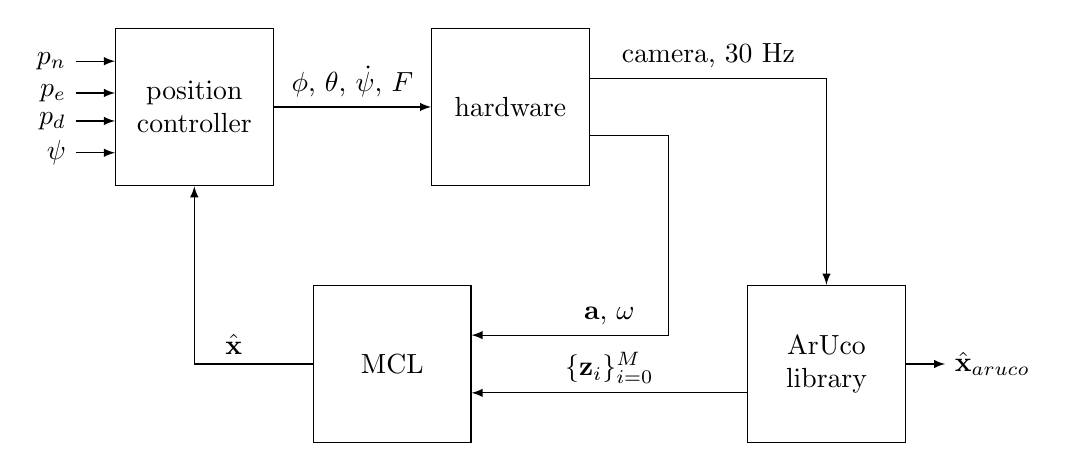
\begin{tikzpicture}[>=latex]

\tikzstyle{block} = [draw, rectangle, align=center, minimum width=2cm, minimum height=2cm]

% Position controller
\node [block] (a) {position\\controller};
\node [left=0.5cm of a.150] (input1) {$p_n$};
\node [left=0.5cm of a.170] (input2) {$p_e$};
\node [left=0.5cm of a.190] (input3) {$p_d$};
\node [left=0.5cm of a.210] (input4) {$\psi$};
\draw [->] (input1) -- (a.150);
\draw [->] (input2) -- (a.170);
\draw [->] (input3) -- (a.190);
\draw [->] (input4) -- (a.210);

% hardware block
\node [block, right=2cm of a] (b) {hardware};
\draw [->] (a) -- node[above] {$\phi$, $\theta$, $\dot{\psi}$, $F$} (b.180);

% ArUco
\node [block, below right=1.25cm and 2cm of b] (c) {ArUco\\library};
\node [right=0.5cm of c] (arucoOut) {$\hat{\mathbf{x}}_{aruco}$};
\draw [->] (b.20) -| node[left=1.5cm, above] {camera, $30$ Hz} (c.90);
\draw [->] (c) -- (arucoOut);

% MCL
\node [block, left=3.5cm of c] (d) {MCL};
\draw [->] (b.340) |- +(1,0) |- node[left=0.75cm, above] {$\mathbf{a}$, $\omega$} (d.20);
\draw [->] (c.200) -- node[above] {$\{\mathbf{z}_i\}_{i=0}^{M}$} (d.340);
\draw [->] (d.180) -| node[right=0.5cm, above] {$\hat{\mathbf{x}}$} (a.270);

\end{tikzpicture}}
    \caption[DesktopQuad system architecture]{DesktopQuad system architecture. Using IMU measurements $\mathbf{a}$ and $\omega$ from the flight controller and ArUco marker pose measurements $\mathbf{z}_i$ from the ArUco library, we perform Monte Carlo localization (MCL) to create a pose estimate $\hat{\mathbf{x}}$ at 100 Hz. This rate is an improvement from the raw ArUco marker map pose estimate $\hat{\mathbf{x}}_{aruco}$ that is created at 20 Hz, which is not sufficient for control.}
    \label{fig:sysarch}
\end{figure}

% !TEX root=main.tex

\section{Quaternions}

A quaternion is a generalization of the complex numbers $a + bi \in \mathbb{C}$. We can think of quaternions as defining a new set $\mathbb{H} = \mathbb{C} + \mathbb{C}j$, and defining $k \triangleq ij$ we create can write any quaternion as
\beq
a + bi + cj + dk \in \mathbb{H}, 
\eeq
where $\{i,j,k\}$ are three imaginary units that multiply as follows:
\beq
i^2 = j^2 = k^2 = ijk = -1.
\eeq

Quaternions are powerful because they share many properties with complex numbers. Regarding quaternions as complex numbers with multidimensional imaginary part, we can rewrite every quaternion,
\beq
q_w + q_xi + q_yj + q_zk = 
\bma
1 & i & j & k
\ema
\bma
q_w \\
q_x \\
q_y \\
q_z \\
\ema
\eeq
We typically refer to this last vector as the quaternion and split it into its real scalar and imaginary vector components
\beq
\mathbf{q} = 
\bma
q_w \\
\mathbf{q}_v \\
\ema
\eeq
Continuing with this notation, we can now create an algebra for quaternions as follows: Let $\mathbf{p},\mathbf{q} \in \mathbb{H}$ and $\alpha \in \mathbb{R}$.
\beq
\alpha\mathbf{q} = 
\bma
\alpha q_w \\
\alpha \mathbf{q}_v
\ema
\eeq
\beq
\mathbf{p} \pm \mathbf{q} = 
\bma
p_w \pm q_w \\
\mathbf{p_v} \pm \mathbf{q_v} \\
\ema
\eeq

\beq
\mathbf{p} \otimes \mathbf{q} =
\bma
p_wq_w - \mathbf{p}_v^\top\mathbf{q}_v \\
p_w\mathbf{q}_v + q_w\mathbf{p}_v + \mathbf{p}_v \times \mathbf{q}_v \\
\ema
\eeq
At this point, we note that 
\beq
\mathbf{p} \otimes \mathbf{q} = - (\mathbf{q} \otimes \mathbf{p})
\eeq
Furthermore, we notice that the quaternion project distributes over the sum
\beq
\mathbf{p} \otimes (\mathbf{q} + \mathbf{r}) = \mathbf{p} \otimes \mathbf{q} + \mathbf{p} \otimes \mathbf{r}
\eeq
\beq
(\mathbf{p} + \mathbf{q}) \otimes \mathbf{r} = \mathbf{p} \otimes \mathbf{r} + \mathbf{q} \otimes \mathbf{r} \\
\eeq


% !TEX root=main.tex

\section{Rigid Body Motion}
When studying rigid body dynamics, we are often concerned with rotations and translations of objects.The configuration space of rigid body is characterized by 6 degrees of freedom, 3 associated with translation and 3 associated with rotation.

\subsection{Coordinate Frames}
Coordinate frames are a useful tool in determining how two rigid bodies are oriented with respect to one another. In the case of UAV work, coodrinate frames are used to determine how a UAV is oriented with respect to a point on the ground. Between two coordinate frames $\mathcal{F}_1, \mathcal{F}_2$, there is an associated rotation $R_1^{2}$ and translation $T_{1 \rightarrow 2}$, transforming the origin of $\mathcal{F}_1$ to $\mathcal{F}_2$. This allows us to take points and vectors in one frame and express them in another frame.

\subsection{Translations}
Translations are often denoted as vectors $T \in \mathbb{R}^3$, which is a vector space. Since $\mathbb{R}^3$ is a vector space, we easily have a global representation of any translation $\mathbf{p}$ given by
\beq
T =
\bma
t_1 \\
t_2 \\
t_3
\ema
\eeq
Now we notice that since points $\mathbf{p}$ also are in $\mathbb{R}^3$, there is a one-to-one correspondence between points and translations, specified by the identity map. We can use this fact to abuse notation and add points and translations (i.e. $\mathbf{p} + T$). Thus, when clear, we will use points and translations interchangeably. 

\subsection{Rotations}
The space of all rotations is denoted by $SO(3)$. These rotations $R \in SO(3)$ are defined as the linear operators $R:\mathbb{R}^3 \rightarrow \mathbb{R}^3$ that perserve vector length and relative orientation of vectors. Specifically let $R:\mathbb{R}^3 \rightarrow \mathbb{R}^3$ and $\mathbf{v},\mathbf{w} \in \mathbb{R}^3$, then we have that
\beq
SO(3) = \{R\ |\ ||R(\mathbf{v})|| = ||\mathbf{v}||, \\R(\mathbf{v})\times R(\mathbf{w}) = \mathbf{v} \times \mathbf{w} \}.
\eeq

The space of rotations has many different representations. One of the most common representations is ZYX euler angles, typically denoted by $(\psi, \theta, \phi)$. This is accomplished by specifying intermediate frames $\mathcal{F}_{\psi}$, $\mathcal{F}_{\psi\theta}$, $\mathcal{F}_{\psi\theta\phi}$. Let $\mathcal{F}_w$ be some fixed intertial reference frame. The intermediate frames are specified as follows
\begin{itemize}
  \item $\mathcal{F}_{\psi}$ results from rotating $\mathcal{F}_w$ about its Z-axis by $\psi$
  \item $\mathcal{F}_{\psi\theta}$ results from rotating $\mathcal{F}_\psi$ about its Y-axis by $\theta$
  \item $\mathcal{F}_{\psi\theta\phi}$ results from rotating $\mathcal{F}_{\psi\theta}$ about its X-axis by $\phi$
\end{itemize}
This representation of rotation is easy to understand and is to understand. However, it suffers from from singularities when the X-axis of $\mathcal{F}_{\psi\theta\phi}$ aligns with the Z-axis of $\mathcal{F}_w$. In these cases, one cannot distinguish between a rotation $\psi$ and $\phi$. Thus, the map from $(\psi, \theta, \phi)$ is not invertible when $\theta = \pm\frac{\pi}{2}$. This scenario is commonly refered to as ``gimbal lock''.

In this work, we will take a more principled approach by taking the definition of $SO(3)$ and applying it to quaternions. We present the following as a candidate rotation operation that takes a vector $\mathbf{v}^1 \in \mathcal{F}_1$ and expresses it in $\mathcal{F}_2$
\beq
\bma
0 \\
\mathbf{v}^2
\ema
= \mathbf{q}_1^2 \otimes 
\bma
0\\
\mathbf{v}^1
\ema \otimes \mathbf{q}_1^{2*}
\eeq
We will denote the operator that performs this operation and extracts $\mathbf{v}^2$ by
\beq
\mathbf{v}^2 = R(\mathbf{q}_1^2)\mathbf{v}^1
\eeq
Imposing the condition $||R(\mathbf{q}_1^2)\mathbf{v}^1|| = ||\mathbf{v}^1||$, we get
\beq
||\mathbf{v}^1|| = ||\mathbf{q}_1^2||^2 ||\mathbf{v}^1||.
\eeq
Thus, we have the additional condition that $||\mathbf{q}_1^2|| = 1$. Note that by the properties of quaternions, relative orientation (i.e. $R(\mathbf{q}_1^2)\mathbf{v}\times R(\mathbf{q}_1^2)\mathbf{w} = \mathbf{v} \times \mathbf{w}$) is also preserved. See Ref. \cite{Sola2017} for more details.

\subsection{Motion}
Now, we will concern ourselves with the change of $R_1^2$ and $T_{1\rightarrow 2}$ over time. To do so, we will specify 3 frames: the world frame $\mathcal{F}_w$, the vehicle frame $\mathcal{F}_v$, and the body frame $\mathcal{F}_b$. Typically in UAV applications, we specify the world frame as an intertial North-East-Down coordinate frame with origin somewhere on the ground. We express the current position of the vehicle $\mathbf{p}^w$ in the world frame. This also happens to be the translation between the world frame and the vehicle frame (i.e. $T_{w\rightarrow v}^w = \mathbf{p}^w$). Typcially we have the the velocity of the vehicle expressed in the body frame $\mathbf{v}^b$. This gives us the kinematic relation
\beq
\dot{\mathbf{p}}^w = \mathbf{v}^w = R(\mathbf{q}_v^{b*})\mathbf{v}^b.
\eeq
This works out nice because the tangent space of $\mathbb{R}^3$ is $\mathbb{R}^3$.

For rotations, we have to determine what is the time derivative of a rotation. Using modern IMUs, we can measure angular velocity $\bm{\omega}_{v \rightarrow b}^{b}$. Ideally, we could express $\dot{\mathbf{q}}_v^b$ as a function of $\bm{\omega}_{v \rightarrow b}^{b}$. We first note that quaternion multiplcation obeys the product rule
\beq
\frac{d}{dt} \mathbf{q} \otimes \mathbf{p} = \dot{\mathbf{q}} \otimes \mathbf{\mathbf{p}} + 
\mathbf{q} \otimes \dot{\mathbf{p}}.
\eeq
Taking the derivative of the unit quaternion constraint, 
\beq
\frac{d}{dt} \mathbf{q}_v^{b*} \otimes \mathbf{q}_v^b = \dot{\mathbf{q}}_v^{b*} \otimes \mathbf{q}_v^{b} + \mathbf{q}_v^{b*} \otimes \dot{\mathbf{q}}_v^b = \mathbf{0}.
\eeq
This implies that
\beq
\mathbf{q}_v^{b*} \otimes \dot{\mathbf{q}}_v^b = -(\mathbf{q}_v^{b*} \otimes \dot{\mathbf{q}}_v^b)^*. 
\eeq
Therefore, $\mathbf{q}_v^{b*} \otimes \dot{\mathbf{q}}_v^b$, must have zero scalar part. Thus, we can rewrite this term as
\beq
\mathbf{q}_v^{b*} \otimes \dot{\mathbf{q}}_v^b = 
\bma
0 \\
\bm{\Omega}
\ema
\eeq
Thus we have the ODE
\beq
\dot{\mathbf{q}}_v^b = \mathbf{q}_v^b \otimes 
\bma
0 \\
\bm{\Omega}
\ema
\eeq
This can be solved using the quaternion exponential 
\beq
\mathbf{q}_v^b(t) = \mathbf{q}_v^b(0) \otimes e^{
\left[0 \ \bm{\Omega} \right]^T}
\eeq
Now we have written the derivative in terms of of some vector $\bm{\Omega} \in \mathbb{R}^3$. We call this the tangent space. Now, we need to determine the relationship between $\bm{\Omega}$ and $\bm{\omega}_{v \rightarrow b}^{b}$. This is given by
\beq
\dot{\mathbf{q}}_v^b = \frac{1}{2}\mathbf{q}_v^b \otimes 
\bma
0 \\
\bm{\omega}_{v \rightarrow b}^{b}
\ema.
\eeq

% !TEX root=main.tex

\section{Kinematics}

\subsection{Nominal State Kinematics}

\beq
\begin{aligned}
  \dot{\mathbf{p}}^w &= R(\mathbf{q}_v^b, \mathbf{v}^b) \\
  \dot{\mathbf{v}}^b &= \mathbf{v} \times \bm{\omega}_{v \rightarrow b}^{b} + \mathbf{a} + 
  R(\mathbf{q}_v^{b*}, \mathbf{g})\\
  \dot{\mathbf{q}}_v^b &= \frac{1}{2} \mathbf{q}_v^b \otimes \bm{\omega}_{v \rightarrow b}^{b}  \\
\end{aligned}
\eeq

\subsection{Error State Kinematics}

\beq
\begin{aligned}
  \dot{\delta \mathbf{p}}^w &= R(\hat{\mathbf{q}}_v^b \otimes \delta \mathbf{q}_v^b, \hat{\mathbf{v}}^b + \delta \mathbf{v}^b) - R(\hat{\mathbf{q}}_v^b, \hat{\mathbf{v}}^b) \\
  \dot{\delta \mathbf{v}}^b &=  \delta \mathbf{v}^b \times \bm{\omega}_{v \rightarrow b}^{b} + R(\delta \mathbf{q}_v^{b*} \otimes \hat{\mathbf{q}}_v^{b*}, \mathbf{g}) - R(\hat{\mathbf{q}}_v^{b*}, \mathbf{g})\\
  \dot{\delta \bm{\theta}} &= \bm{\omega}_{v \rightarrow b}^{b} \times \delta \bm{\theta}\\
    \delta \mathbf{q}_v^b &= e^{\delta \bm{\theta} / 2}
\end{aligned}
\eeq

%% !TEX root=main.tex

\section{Motion Models}
\label{sec:motion_models}
In order to achieve a high rate of state estimates, it is important to propagate the position and orientation state of the micro quad in between measurement updates. In this project, two types of motion models were implemented and compared.

\begin{equation}
\x \triangleq
\begin{pmatrix}
\p^\top & {\q_W^C}^\top & \v^\top & \angvel^\top
\end{pmatrix}
^\top
\end{equation}

\subsection{Stochastically-Driven Nearly-Constant Velocity}
\label{subsec:mm-sndcv}

The first motion model used is a 6 degree of freedom (DOF) nearly-constant velocity model, driven by linear and angular acceleration noise processes.

\begin{equation}
\x[\dot] =
\begin{pmatrix}
\p[\dot] \\ \q[\dot]_W^C \\ \v[\dot] \\ \angvel[\dot]
\end{pmatrix}
=
\begin{pmatrix}
\v \\ \frac{1}{2} \q \otimes \q\of{\angvel} \\ \accel \\ \angcel
\end{pmatrix}
\end{equation}

\begin{align}
\accel &\sim \mathcal{N}\of{\0,\Q_{\accel}} \\
\angcel &\sim \mathcal{N}\of{\0,\Q_{\angcel}}
\end{align}

where $\accel \sim \mathcal{N}\of{\0,\Q_{\accel}}$ and $\angcel \sim \mathcal{N}\of{\0,\Q_{\angcel}}$ and are wide-sense stationary (WSS).

\subsection{IMU Mechanized}
\label{subsec:mm-mech}

To overcome the issues of the SDNCV motion model, an IMU mechanized motion model is introduced that takes into account quadrotor kinematics \cite{Beard2008}.

\begin{equation}
\x[\dot] =
\begin{pmatrix}
\p[\dot] \\ \q[\dot]_W^C \\ \v[\dot] \\ \angvel[\dot]
\end{pmatrix}
=
\begin{pmatrix}
\v \\ \frac{1}{2} \q \otimes \q\of{\angvel} \\ \accel \\ -
\end{pmatrix}
\end{equation}

where $\accel$ and $\angvel$ come from the IMU as measurements.



\addtolength{\textheight}{-4.5cm}   % This command serves to balance the column lengths
                                  % on the last page of the document manually. It shortens
                                  % the textheight of the last page by a suitable amount.
                                  % This command does not take effect until the next page
                                  % so it should come on the page before the last. Make
                                  % sure that you do not shorten the textheight too much.

\bibliographystyle{ieeetr}
\bibliography{refs}

\end{document}
